% Solution to the Lecture 1 mini case (slides 31-33 of Aula/Lecture01.pdf): where to open the pharmacy?
% Compile: pdflatex mini-case-lecture-01.tex (twice). Check: pdffonts (all Type 1, uni = yes).
% Every number is asserted by mini-case-lecture-01-check.py in this folder.
\documentclass[11pt,a4paper]{article}
\usepackage[utf8]{inputenc}
\usepackage[T1]{fontenc}
\usepackage{lmodern}   % Type 1 vector fonts (replaces PK bitmaps)
\usepackage{cmap}      % ToUnicode CMap -> copyable text and accents
\usepackage[english]{babel}
\usepackage{amsmath,amssymb,amsthm,mathtools}
\usepackage[a4paper,margin=2.4cm]{geometry}
\usepackage{microtype}
\usepackage{booktabs,array}
\usepackage{enumitem}
\usepackage{xcolor}
\usepackage{tikz}
\usepackage[most]{tcolorbox}
\usepackage{fancyhdr}
\usepackage[hidelinks]{hyperref}

\setlist{topsep=3pt,itemsep=2pt}
\setlength{\parindent}{0pt}
\setlength{\parskip}{5pt}
\renewcommand{\arraystretch}{1.2}
\allowdisplaybreaks

\pagestyle{fancy}\fancyhf{}
\lhead{\footnotesize Economics of Organizations and Incentives --- MPE Insper}
\rhead{\footnotesize Lecture 1 mini case: solution}
\cfoot{\footnotesize\thepage}
\renewcommand{\headrulewidth}{0.3pt}
\setlength{\headheight}{14pt}

\definecolor{ans}{RGB}{20,110,70}
\definecolor{src}{RGB}{30,80,150}
\newcommand{\answer}[1]{\begin{tcolorbox}[colback=ans!5,colframe=ans,boxrule=0.6pt,
  left=5pt,right=5pt,top=3pt,bottom=3pt]\textbf{Answer.} #1\end{tcolorbox}}
\newenvironment{notacao}{\par\smallskip\noindent\textbf{Notation.}\begin{itemize}[leftmargin=1.4em,topsep=1pt,itemsep=0pt]\small}{\end{itemize}}

\title{\textbf{Mini Case, Lecture 1: Where to Open the Pharmacy?}\\[4pt]
  \large Solution --- Economics of Organizations and Incentives (MPE Insper)}
\date{October 2026}

\begin{document}
\maketitle
\thispagestyle{empty}

\section*{The case}

\textbf{Source.} Lecture 1 slides (\texttt{Aula/Lecture01.pdf}), slides 32--33, ``Mini case: where to
open the pharmacy?'' and ``Mini case: questions''; motivation on slide 31 (Revista PEGN, 2023, a
pharmacy rivalry in Brasília). Reproduced verbatim.

\begin{tcolorbox}[colback=src!4,colframe=src,boxrule=0.5pt]
Two pharmacy chains, A and B, will each open one store on a new avenue with 7 blocks.

\begin{center}
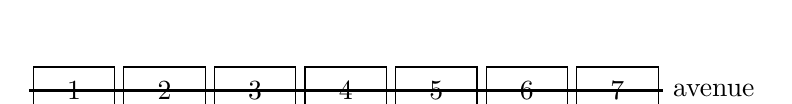
\begin{tikzpicture}[x=1.15cm]
  \draw[thick] (0.5,0) -- (7.5,0) node[right] {avenue};
  \foreach \b in {1,...,7} { \draw (\b-0.45,-0.3) rectangle (\b+0.45,0.3); \node at (\b,0) {\b}; }
\end{tikzpicture}
\end{center}

Each block has the same number of customers (normalize to 1 per block).

Both chains choose a block simultaneously. Prices and products are identical.

Customers buy from the nearest store and split evenly if both are equally distant.

Each chain maximizes its number of customers.

\medskip
\textbf{Mini case: questions (in pairs, hand in today)}
\begin{enumerate}[label=(\alph*)]
  \item Write the game in normal form. Give a formula for $u_A(s_A, s_B)$ when $s_A < s_B$,
        $s_A = s_B$ and $s_A > s_B$.
  \item Show that block 1 is strictly dominated by block 2. Is any block strictly dominant?
  \item Apply IESDS. Describe each round. Which location profile survives?
  \item Customers dislike walking. Which pair of locations minimizes the total distance walked?
        Compare with your answer in (c).
  \item Which assumptions drive your prediction? What would change if the chains also chose
        prices? Give a real-world example of clustering, or of firms spreading out.
\end{enumerate}
\end{tcolorbox}

\textbf{Method.} Normal form (slides 13--14), strict dominance (slide 23) and IESDS
(slides 28--29); Tadelis (2013) \S3.2 (pp.~47--52), \S4.1 (pp.~59--63), \S4.2 (pp.~63--69). The
case is the discrete Hotelling location game; Tadelis Exercise~4.10 (p.~78) is its five-tower
version. Every number below is asserted by \texttt{Resolucao/mini-case-lecture-01-check.py}.

\begin{notacao}
  \item $I = \{A, B\}$: the two chains (players).
  \item $s_A, s_B \in \{1, \dots, 7\}$: the block where each chain opens its store.
  \item $j \in \{1, \dots, 7\}$: a block of customers (one customer per block, 7 in total).
  \item $u_A(s_A, s_B)$: customers served by A, a multiple of $\tfrac12$ in $[\tfrac12, 6]$.
  \item $m = (s_A + s_B)/2$: the midpoint between the stores; an integer or a half-integer.
  \item $S_i^k$: chain $i$'s blocks that survive $k$ rounds of IESDS; $S_i^0 = \{1, \dots, 7\}$.
  \item $W(x, y)$: total blocks walked by customers when the stores are at $x \le y$.
\end{notacao}

%-------------------------------------------------------------------------------------------
\section*{(a) Normal form and the payoff formula}

The game is $G = (I, \{S_i\}_{i \in I}, \{u_i\}_{i \in I})$ with $I = \{A, B\}$ and
$S_A = S_B = \{1, 2, \dots, 7\}$. Payoffs follow from where each customer buys.

\textbf{Case $s_A < s_B$.} A customer at block $j \le s_A$ is closer to A. A customer between the
stores, $s_A < j < s_B$, compares $j - s_A$ with $s_B - j$:
\begin{align}
  j - s_A &< s_B - j \nonumber\\
  2j &< s_A + s_B \nonumber\\
  j &< m. \label{eq:closer}
\end{align}
By \eqref{eq:closer}, A serves every block $j < m$ and half of block $j = m$ when $m$ is an
integer. If $m$ is an integer, that is $m - 1$ whole blocks plus one half:
\begin{equation}
  u_A = (m - 1) + \tfrac12 = m - \tfrac12. \label{eq:mint}
\end{equation}
If $m$ is a half-integer, A serves blocks $1, \dots, m - \tfrac12$, so again $u_A = m - \tfrac12$.
Substituting $m = (s_A + s_B)/2$ into \eqref{eq:mint}:
\begin{align}
  u_A &= \Big(\frac{s_A + s_B}{2}\Big) - \frac12 \nonumber\\
      &= \frac{s_A + s_B - 1}{2}. \label{eq:left}
\end{align}

\textbf{Case $s_A = s_B$.} Every customer is equally distant, so each chain gets half of the 7.

\textbf{Case $s_A > s_B$.} Every customer buys from one store, so $u_A + u_B = 7$ in every cell
(the game is constant-sum). B is now the left store, so \eqref{eq:left} with the roles swapped
gives $u_B = (s_B + s_A - 1)/2$. Substituting into $u_A = 7 - u_B$:
\begin{align}
  u_A &= 7 - \Big(\frac{s_A + s_B - 1}{2}\Big) \nonumber\\
      &= \frac{15 - s_A - s_B}{2}. \label{eq:right}
\end{align}

Collecting \eqref{eq:left}, the tie and \eqref{eq:right}:
\begin{equation}
  u_A(s_A, s_B) =
  \begin{cases}
    \dfrac{s_A + s_B - 1}{2} & \text{if } s_A < s_B,\\[6pt]
    \dfrac{7}{2} & \text{if } s_A = s_B,\\[6pt]
    \dfrac{15 - s_A - s_B}{2} & \text{if } s_A > s_B,
  \end{cases}
  \qquad u_B(s_A, s_B) = u_A(s_B, s_A). \label{eq:payoff}
\end{equation}
\emph{Check of one cell.} $(s_A, s_B) = (2, 6)$: $u_A = (2 + 6 - 1)/2 = 3.5$. By hand, A
serves blocks 1, 2, 3 and half of block 4 (two blocks from each store): $3 + 0.5 = 3.5$.

A's payoffs (rows $s_A$, columns $s_B$); B's payoff in each cell is $7$ minus A's:
\begin{center}
\begin{tabular}{c|ccccccc}
$s_A \backslash s_B$ & 1 & 2 & 3 & 4 & 5 & 6 & 7 \\ \midrule
1 & 3.5 & 1   & 1.5 & 2   & 2.5 & 3   & 3.5 \\
2 & 6   & 3.5 & 2   & 2.5 & 3   & 3.5 & 4   \\
3 & 5.5 & 5   & 3.5 & 3   & 3.5 & 4   & 4.5 \\
4 & 5   & 4.5 & 4   & 3.5 & 4   & 4.5 & 5   \\
5 & 4.5 & 4   & 3.5 & 3   & 3.5 & 5   & 5.5 \\
6 & 4   & 3.5 & 3   & 2.5 & 2   & 3.5 & 6   \\
7 & 3.5 & 3   & 2.5 & 2   & 1.5 & 1   & 3.5
\end{tabular}
\end{center}

\answer{$G = (\{A,B\}, \{S_A = S_B = \{1,\dots,7\}\}, \{u_A, u_B\})$ with $u_A$ given by
\eqref{eq:payoff}: $(s_A + s_B - 1)/2$ if $s_A < s_B$, $7/2$ if $s_A = s_B$, $(15 - s_A - s_B)/2$ if
$s_A > s_B$; and $u_B = 7 - u_A$.}

%-------------------------------------------------------------------------------------------
\section*{(b) Block 1 is strictly dominated by block 2; no block is strictly dominant}

Block 2 strictly dominates block 1 for A if $u_A(2, s_B) > u_A(1, s_B)$ for \emph{every}
$s_B \in \{1, \dots, 7\}$: seven inequalities.

\emph{$s_B = 1$.} Block 1 ties; block 2 is to the right, so \eqref{eq:right} applies:
\begin{align*}
  u_A(1, 1) &= 3.5,\\
  u_A(2, 1) &= \frac{15 - (2) - (1)}{2} = 6 > 3.5.
\end{align*}
\emph{$s_B = 2$.} Block 1 is to the left, \eqref{eq:left}; block 2 ties:
\begin{align*}
  u_A(1, 2) &= \frac{(1) + (2) - 1}{2} = 1,\\
  u_A(2, 2) &= 3.5 > 1.
\end{align*}
\emph{$s_B \ge 3$.} Both blocks are to the left of B, so \eqref{eq:left} applies to both:
\begin{align}
  u_A(1, s_B) &= \frac{(1) + s_B - 1}{2} = \frac{s_B}{2}, \nonumber\\
  u_A(2, s_B) &= \frac{(2) + s_B - 1}{2} = \frac{s_B + 1}{2}, \nonumber\\
  u_A(2, s_B) - u_A(1, s_B) &= \frac{s_B + 1}{2} - \frac{s_B}{2} = \frac12 > 0. \label{eq:gain}
\end{align}
All seven inequalities hold (gains $2.5, 2.5, 0.5, 0.5, 0.5, 0.5, 0.5$), so block 1 is strictly
dominated by block 2. By the symmetry of the avenue, block 7 is strictly dominated by block 6;
the same holds for B. \eqref{eq:gain} has an intuition: moving one block inward keeps every
customer A had and wins half a block more from the rival.

\textbf{No strictly dominant block.} A strictly dominant block would have to be the unique best
reply to \emph{every} $s_B$. From the matrix, the best reply to $s_B = 1$ is block 2 only
($u_A = 6$), and the best reply to $s_B = 4$ is block 4 only ($u_A = 3.5$; every other block gets
at most $3$). Block 2 loses to block 4 when $s_B = 4$, and every block other than 2 loses to
block 2 when $s_B = 1$. One counterexample cell per candidate is enough.

\answer{Block 2 beats block 1 against all seven rival choices (by $2.5$ when $s_B \le 2$, by
$\tfrac12$ when $s_B \ge 3$), so block 1 is strictly dominated (and block 7 by block 6). No block is
strictly dominant: the best reply to $s_B = 1$ is block 2 and to $s_B = 4$ is block 4.}

%-------------------------------------------------------------------------------------------
\section*{(c) IESDS}

Each round removes every block that is strictly dominated given the rival blocks still alive. A
block that is the unique best reply to some surviving rival block cannot be strictly dominated, so
it stays; from the matrix, the best replies are
$1 \mapsto 2,\ 2 \mapsto 3,\ 3 \mapsto 4,\ 4 \mapsto 4,\ 5 \mapsto 4,\ 6 \mapsto 5,\ 7 \mapsto 6$.

\textbf{Round 1} (rivals in $S_B^0 = \{1, \dots, 7\}$). Blocks 1 and 7 are strictly dominated,
by 2 and 6 (part (b)). Blocks 2--6 are best replies to $1, 2, 4, 6, 7$, so they stay. Both
chains face the same problem:
\[
  S_A^1 = S_B^1 = \{2, 3, 4, 5, 6\}.
\]
\emph{Knowledge used:} only that each chain is rational.

\textbf{Round 2} (rivals in $\{2, \dots, 6\}$). Rows 2 and 3 of the matrix, columns 2--6:
\begin{center}
\begin{tabular}{c|ccccc}
$s_A \backslash s_B$ & 2 & 3 & 4 & 5 & 6 \\ \midrule
2 & 3.5 & 2 & 2.5 & 3 & 3.5 \\
3 & 5 & 3.5 & 3 & 3.5 & 4
\end{tabular}
\end{center}
Block 3 is larger in every column, so block 2 is strictly dominated by 3; symmetrically, 6 by 5.
Blocks 3, 4, 5 are best replies to $2, 4, 6$, which are still alive, so they stay:
\[
  S_A^2 = S_B^2 = \{3, 4, 5\}.
\]
\emph{Knowledge used:} A knows that B is rational. Against $s_B = 1$ block 2 beats block 3
($u_A(2, 1) = 6 > 5.5 = u_A(3, 1)$), so A can drop block 2 only after ruling out $s_B = 1$.

\textbf{Round 3} (rivals in $\{3, 4, 5\}$):
\begin{center}
\begin{tabular}{c|ccc}
$s_A \backslash s_B$ & 3 & 4 & 5 \\ \midrule
3 & 3.5 & 3 & 3.5 \\
4 & 4 & 3.5 & 4 \\
5 & 3.5 & 3 & 3.5
\end{tabular}
\end{center}
Block 4 beats blocks 3 and 5 in every column:
\[
  S_A^3 = S_B^3 = \{4\}.
\]
\emph{Knowledge used:} A knows that B knows that A is rational. Against $s_B = 2$ block 3 beats
block 4 ($5 > 4.5$), so A drops block 3 only after ruling out $s_B = 2$, which B dropped in
round 2 because B knows A is rational.

Nothing is left to remove, so $S^\infty = \{(4, 4)\}$, with payoffs
\[
  u_A(4, 4) = u_B(4, 4) = \tfrac72.
\]

\answer{Round 1 removes $\{1, 7\}$, round 2 removes $\{2, 6\}$, round 3 removes $\{3, 5\}$ (for
both chains). The unique surviving profile is $(4, 4)$: both pharmacies open on the middle block,
side by side, and each serves $3.5$ customers. It takes rationality plus two levels of knowledge
of rationality. (Lecture 2 preview: $(4,4)$ is also the unique Nash equilibrium.)}

%-------------------------------------------------------------------------------------------
\section*{(d) The locations that minimize total walking}

With the stores at $x \le y$, each customer walks to the nearer store:
\begin{equation}
  W(x, y) = \sum_{j=1}^{7} \min\{|j - x|, |j - y|\}. \label{eq:walk}
\end{equation}

\textbf{Lower bound.} Any pair of stores splits the avenue into a left group of $k$ consecutive
blocks (served by $x$) and a right group of $7 - k$ blocks. For a group of $n$ consecutive blocks
served by one store, total walking is smallest with the store at the group's median, where it
equals $\lfloor n^2/4 \rfloor$ (for $n = 3$: $1 + 0 + 1 = 2$; for $n = 4$: $1 + 0 + 1 + 2 = 4$).
So
\begin{equation}
  W(x, y) \ge \Big\lfloor \frac{k^2}{4} \Big\rfloor + \Big\lfloor \frac{(7 - k)^2}{4} \Big\rfloor.
  \label{eq:bound}
\end{equation}
Evaluating \eqref{eq:bound} for each split:
\begin{center}
\begin{tabular}{c|cccccccc}
$k$ & 0 & 1 & 2 & 3 & 4 & 5 & 6 & 7 \\ \midrule
$\lfloor k^2/4\rfloor + \lfloor (7-k)^2/4\rfloor$ & 12 & 9 & 7 & 6 & 6 & 7 & 9 & 12
\end{tabular}
\end{center}
The minimum is 6, at the splits $3 + 4$ and $4 + 3$, so no pair walks less than 6.

\textbf{Attaining it.} Split $3 + 4$: blocks 1--3 served from their median, block 2; blocks
4--7 from a median, block 5 or 6. Substituting $(x, y) = (2, 6)$ into \eqref{eq:walk}, block by
block from $j = 1$:
\begin{align*}
  W(2, 6) &= 1 + 0 + 1 + 2 + 1 + 0 + 1\\
          &= 6.
\end{align*}
A brute-force search over all 28 pairs (check script) gives exactly three minimizers:
$\{2, 5\}$, $\{2, 6\}$ and $\{3, 6\}$.

\textbf{Comparison with (c).} Substituting $(x, y) = (4, 4)$ into \eqref{eq:walk}:
\begin{align*}
  W(4, 4) &= 3 + 2 + 1 + 0 + 1 + 2 + 3\\
          &= 12,
\end{align*}
twice the minimum. Competition puts both stores in the middle; customers would be better served
by stores spread to about the quartiles of the avenue. The chains do not care: the game is
constant-sum ($u_A + u_B = 7$ in every cell), so every profile, $(4, 4)$ included, is Pareto
optimal \emph{for the two chains}, and that says nothing about customers. Nor is the efficient
pair self-enforcing: at $(2, 6)$ each chain gets $3.5$, but A moving from 2 to 3 gets
\[
  u_A(3, 6) = \frac{(3) + (6) - 1}{2} = 4 > 3.5,
\]
so each chain creeps toward the centre until both stand at block 4.

\answer{Total walking is minimized (6 blocks) at $\{2, 5\}$, $\{2, 6\}$ or $\{3, 6\}$, about one
store per half of the avenue. The IESDS profile $(4, 4)$ makes customers walk 12, twice as much.
The chains' rivalry is constant-sum, so the extra walking is a pure loss to customers with no
gain to the chains as a group, yet neither chain can resist moving inward.}

%-------------------------------------------------------------------------------------------
\section*{(e) Assumptions, prices, and examples}

\textbf{Assumptions that drive ``meet in the middle''.}
\begin{itemize}
  \item \emph{Fixed, identical prices and products.} The chains compete only on location, so the
        only way to win customers is to stand closer to more of them. This is the key one (see
        prices below).
  \item \emph{Inelastic demand.} Every customer buys whatever the distance, so moving toward the
        centre never loses the customers at the ends. If far customers stopped buying, a chain
        at the centre would lose its ends and the pull to the middle would weaken.
  \item \emph{Two chains, one store each, on a line.} With three stores the middle store is
        squeezed from both sides and the clustering prediction breaks down; with more stores per
        chain, chains spread their own stores out.
  \item \emph{Uniform customers.} With an uneven avenue the stores still meet, but at the median
        customer, not the middle block.
  \item \emph{Simultaneous, once-and-for-all choice; customers go to the nearest store}
        (no brand loyalty or other differences).
\end{itemize}

\textbf{If the chains also chose prices.} Then two stores on the same block sell identical
products at the same spot, so they compete as in Bertrand: prices fall to marginal cost and
profits to zero. Location becomes a way to soften price competition, and the chains now have a
reason to move \emph{apart}. In Hotelling's linear city with quadratic transport costs and
locations chosen before prices, the firms locate at the two ends of the line (maximal
differentiation; d'Aspremont, Gabszewicz and Thisse, 1979). Reading: Cabral (2017) \S14.2
(pp.~354, 358--360). The prediction flips from minimal to maximal differentiation once prices
are a choice.

\textbf{Real-world examples.}
\begin{itemize}
  \item \emph{Clustering:} the competing pharmacies on the same Brasília street (slide 31);
        competing petrol stations at the same junction; fast-food chains next to each other;
        two-party platforms converging on the median voter (Hotelling 1929, Downs 1957). Medicine
        prices in Brazil are capped by a regulator (CMED) and pharmacies carry similar products,
        which brings the case closer to the ``fixed, identical prices'' assumption than most
        retail.
  \item \emph{Spreading out:} a single chain placing its own stores in different neighbourhoods
        (it does not compete with itself), and sellers who compete hard on price, where staying
        apart protects margins.
\end{itemize}

\answer{The clustering result rests on fixed identical prices, inelastic demand, two single-store
firms and nearest-store shopping. Allowing price choice reverses it: side by side, the stores
would face Bertrand competition, so they spread out to soften it. Clustering: pharmacies in
Brasília, petrol stations, political platforms. Spreading out: a chain's own branches, and firms
in price-sensitive markets.}

\end{document}
